\documentclass[FM,BP]{tulthesis}
% tento dokument používá balíky specifické pro XeLaTeX a lze jej přeložit
% jen XeLaTeXem, nemáte-li instalována použitá (komerční) písma, změňte
% nebo vymažte příkazy \set...font na následujících řádcích

\newcommand{\verze}{1.7}

\usepackage{polyglossia}
\setdefaultlanguage{czech}
\usepackage{xevlna}

\usepackage{makeidx}
\makeindex

% fonty
\usepackage{fontspec}
\usepackage{xunicode}
\usepackage{xltxtra}
\usepackage{graphicx}


% příkazy specifické pro tento dokument
\newcommand{\argument}[1]{{\ttfamily\color{\tulcolor}#1}}
\newcommand{\argumentindex}[1]{\argument{#1}\index{#1}}
\newcommand{\prostredi}[1]{\argumentindex{#1}}
\newcommand{\prikazneindex}[1]{\argument{\textbackslash #1}}
\newcommand{\prikaz}[1]{\prikazneindex{#1}\index{#1@\textbackslash #1}}
\newenvironment{myquote}{\begin{list}{}{\setlength\leftmargin\parindent}\item[]}{\end{list}}
\newenvironment{listing}{\begin{myquote}\color{\tulcolor}}{\end{myquote}}
\sloppy

% deklarace pro titulní stránku

\TULtitle{Vizualizace a tvorba analýz z dat v oblasti kvality a kvantity odběru elektrické energie}{Visualization and analysis of data in the field of quality and quantity of electricity}
\TULprogramme{B2646}{Informační technologie}{Information technology}
\TULbranch{1802R007}{Informační technologie}{Information technology}
\TULauthor{Jan Špecián}
\TULsupervisor{Ing. Jan Kraus Ph.D.}
\TULyear{2019}

\begin{document}
\ThesisTitle{EN}
\ThesisStart{pic/zadaniBPScan.pdf}

\begin{abstractEN}
    Práce je zaměřena na přípravu softwarového nástroje pro tvorbu automatických analýz dat získaných z chytrého elektroměru od firmy KMB Systems s.r.o. Jsou zde uvedeny příklady v praxi nejčastěji používaných přehledových spojnicových grafů. Následně jsou jsou zde probrány dostupné softwarové technologie pro vývoj příslušné webové aplikace a jejich použití pro tvorbu přehledové nástěňky vygenerované z naměřených dat za pomoci uživatelsky definovatelných šablon a export výsledků do pdf.
\end{abstractEN}

\begin{keywordsEN}
    Energy management system, PQ monitor, REST API, sledování spotřeby elektrické energie
\end{keywordsEN}

\begin{abstractCZ}
    The goal of the thesis is to develop a software tool for creating and managing visual analysis on data collected by a smart meter device from KMB Systems s.r.o. There are examples of most frequently used line graphs. Subsequently there are available software technologies for the development of web application and their use for the creation of the overview board generated from the measured data with respect to user definable templates and export the results to pdf.
\end{abstractCZ}


\begin{keywordsCZ}
    Energy management system, PQ monitor, REST API, monitoring of electricity consumption
\end{keywordsCZ}

\vspace{2cm}



\clearpage

\begin{acknowledgement}
    Tímto bych rád poděkoval Ing. Janu Krausovi, Ph.D. za věnovaný čas v konzultacích a odborné vedení plné trpělivosti a s tím spojené nabyté zkušenosti.
\end{acknowledgement}

\tableofcontents
\listoffigures

\clearpage

\begin{abbrList}
    \textbf{EF} & Entity Framework \\
    \textbf{JSON} & JavaScript Object Notation \\
    \textbf{LINQ} & Language Integrated Query \\
    \textbf{NPM} & Node Package Manager \\
    \textbf{wysiwyg} & What you see is what you get \\
    \textbf{DI} & Dependency Injection \\
    \textbf{SQL} & Structured Query Language \\
    \textbf{MVC} & Model-View-Controller \\
    \textbf{API} & Application Program Interface \\
    \textbf{CSS} & Cascade Style Sheets \\
    \textbf{PDF} & Portable Document Format \\
   
\end{abbrList}

\chapter*{Úvod}
    Úkolem bákalářské práce je vytvoření webové aplikace pro uživatelsky příjemné a přehledné a definovatelné zobrazení nástěnky 
    z naměřených dat chytrými elektroměry firmy KMB systems s.r.o. 
    Jak je možno vidět z archivů elektrické energie, tyto přístroje měří stovky veličin periodicky v intervalu 
    jednotek sekund a tím poskytují detailní přehled o odběru elektrické energie a její kvality na základě sepnuté zátěže.

    Hlavní motivací je vytvořit z naměřených dat přehlednou nástěnku nejen ve formě webové stránky, 
    ale i reportu ve formátu pdf, kde by zákazník viděl průběhy naměřených veličin za dané období ve formě spojnicových, 
    koláčových grafů, či tabulek. 
    Archivované průběhy veličin mohou pomoci najít vztah mezi spínáním velké zátěže a poruch 
    na jiných přístrojích v síti, či pomoci s rozložením zátěže do vhodných tarifních časových pásem.

    Definovatelný report může být detailní a zobrazovat hodnoty tak jak byly změřeny, 
    ale naopak může zobrazovat ryze přehledové grafy a tabulky s průměry a maximy apod. 
    Průběhy a hodnoty, které zákazníka zajímají si sám nadefinuje a může je opakovaně prohlížet. 
    Takto definovaný report lze použít jako automaticky generovaný přehled a odesílat zákazníkovi 
    ve formě pdf jako notifikace k problému v síti, překročení limitů, či pouze pro pravidelný přehled. 
    Reporty mohou být běžným doplňkem ke každému chytrému elektroměru ať už v domácosti, či velkém průmyslovém provozu.

    V první části zprávy uvedu přehled existujících řešení o jiných firem a existující knihovny pro tvorbu grafů v klientské aplikaci, tak pro tvorbu pdf. 
    Výber použitých technologií a postup zpracování naměřených dat.
    Praktická část ukazuje průběh návrhu a implementace serverové a klientské části webové aplikace, 
    průběh zpracování dat v serverové části aplikace při volání API a pomocných třídách a použití nejnovějších technologií k tvorbě klientské části.

\chapter{Teoretická část}
    \section{Energetický management}
        Energetický management je definován jako soubor opatření, jejichž cílem je efektivní řízení a snižování spotřeb energií. \cite{30}
        Pro detailní záznam a analýzu spotřeby energií se využívá informačních technologií.
        IT systém umožňuje sledování toků veškerých toků energií a jejich nákladů, \cite{30}
        Hlavním důvodem pro implementaci systému EnMS dle normy ČSN EN ISO 50001 do společnosti jsou stálé a systematické energetické úspory.
        Toho lze dosáhnout optimalizací spotřeb energie a jiných médií, optimalizací výroby a dodávky energie.\cite{31}
    \section{Typické veličiny zaznamenané v archivu chytrého elektroměru}
        Veličiny zaznamenané v archivu jsou definovány v normě IEEE1459-2010 s názvem 
        IEEE Standard Definitions for the Measurement of Electric Power Quantities Under Sinusoidal, Nonsinusoidal, Balanced, or Unbalanced Conditions. 
        Konkrétně se jedná o výkon (činný, jalový, zdánlivý), napětí, proud, frekvenci, vzájemný posun fází v třífázové soustavě. 
        Dále .cea archiv obsahoval stavové veličiny indikující sepnutí různých zátěží v čase a teplotu. 
        Vektor těchto hodnot je zaznamenáván periodicky, obvykle v pevném intervalu od desítek milisekund 
        po jednotky sekund a ukládán do paměti měřícího přístroje. 
        Archiv elektrické energie může obsahovat stovky hodnot naměřených periodicky, obvykle jednotky sekund.
        Zažízení poskytuje možnost archivace dat v paměti a její odesílání v dávkách do vzdáleného úložiště. 
        Dále mohou být významné statusové hodnoty 0/1 v porovnání s naměřenými veličinami 
        pro monitorování kvality elektrické energie při spínání různě velké zátěže. 
        Konkrétní archivy poskytnuté pro testování aplikace měly periodu záznamu 10sekund.
    \section{Možnosti ukládání dat z archivu elektrické energie}
        \subsection*{CSV}
            Jedná se o nejjednodušší formát ukládání časových řad ve dvojrozměrné tabulce. 
            Snadno zpracovatelný a modifikovatelný soubor, kde jsou hodnoty v textovém souboru rozdělené separátorem, obvykle středníkem, nebo čárkou. 
        \subsection*{JSON}
            Javascriptový zápis objektů ve složených závorkách a polí v hranatých závorkách umožňuje zapsat libovolně zanořené a komplikované struktury. 
            V mé bakalářské práci je tento formát použit pro posílání dat mezi klientskou a serverovou částí.
        \subsection*{.CEA}
            Výše uvedené formáty jsou univerzální formáty pro výměnu dat. 
            Tento formát používá firma KMB Systems s.r.o. pro archivaci dat ve svých chtyrých elektorměrech. 
            Pro vizualizaci uložených dat je možno použít desktopovou aplikaci Envis a pro čtení časových řad je 
            potřeba použít speciálních knihoven od KMB pro .NET Framework verze 4.5.2 a vyšší.

    \section{Vhodná technologie pro vývoj webových služeb}
        KMB knihovna pro čtení .cea dat i aplikace envis pro podrobnou vizualizaci dat v .cea souborech jsou vyvíjené pod .NET Standard 2.0, proto je 
        i tato webová aplikace ve stejném frameworku. 
        Případné použítí součástí aplikace pro začlenění nástrojů včetně definovatelných reportů a pdf exportu do existujícího KMB ekosystému bude nejsnažší. 

    \section{Použité technologie}
        \subsection{Serverová část}
            \subsubsection{ASP.NET Core 2.x}
                Architektura ASP.NET Core MVC je open-source framework umožňující vytvářet webová rozhraní API a webové aplikace v jazyce C\#. 
                Sjednocuje dříve separátní ASP.NET MVC a ASP.NET Web API pod jeden framework. 
                Došlo ke změně přístupu ve vývoji asp.net webových frameworků směrem k modulárnosti namísto snahy poskytnout veškerou funkcionalitu v jednom velkém frameworku. 
                Veškeré části .net Core jsou samostatné NuGet balíky a vývojář si může vybrat, které balíky použije. 
                Existují agregační balíky, které obsahují sadu souvisejících balíků, tak aby vývojář nemusel referencovat jednotlivé balíky a knihovny.\cite{1}

                Je primárně určen pro vývoj webových aplikací. 
                Společně s .net core byla vydána sada Extension knihoven pro často potřebné úlohy, jako je logování, konfigurace, dependency injection container, či caching. 
                Hlavní sada knihoven pro obsluhu volání API je ASP.NET MVC Core poskytující architekturu pro vytváření webových aplikací a rozhraní API pomocí Model-View-Controller návrhu. \cite{1}

                Webová aplikace v .net core narozdíl od klasického asp.net framworku je modulární a není potřeba mít nainstalovaný plný .net framework.

            \subsubsection{Entity framework}
                Umožňuje práci s daty na vyšší úrovni, oproti dotazování se do databáze za pomoci sql dotazů. 
                Jedná se o objektově-relační mapovací technologii umožňující pracovat s databázovými tabulkami jako s objekty .net a tím vynechat množství kódu pro přístup k datům. 
                Model je tvořen třídami entit a objektem kontextu DbContext, který představuje spojení s databází a poskytuje možnost data získávat i upravovat. 
                Model může být vygenerován z existující databáze, nebo naopak z vytvořeného objektového modelu může být vygenerována prázdná databáze.
                Anotace atributů lze najít v dokumentaci, nejčastějším důvodem jejich použítí je speciální požadavek na sloupec.
                V modelových třídách je možno mít počítané nemapované atributy uvedené anotací [NotMapped], či pomocí anotace [MaxLength(500)] 
                určit maximální délku řetězce v daném sloupci tabulky a další.
                \cite{4}

            \subsubsection{Migrace v EF}
                V průběhu vývoje aplikace se často objeví potřeba změnit databázový model. Přidat, či odebrat entity, atributy, nebo cizí klíče.
                Prvním přístupem je smazání databáze se všemi informacemi a vytvoření nové podle nového upraveného modelu.
                Druhou možností je použít Migrace v .NET Core poskytující možnost postupně upravovat model a synchronizovat databázi tak, aby nedošlo ke ztrátě dat.
                Každá migrace obsahuje metody Up() a Down(), které obsahují definice pro úpravu databáze pro možnost návratu zpět k předchozímu stavu modelu. 
                \cite{23}

            \subsubsection{Linq}
                Knihovna posktující přehlednou a kompaktní syntaxi pro manipulaci s daty. 
                Lze vytvořit dotaz nad různými typy dat nezávisle nad dotazovaným zdrojem dat, kterým může být SQL databáze, pole objektů, či XML. 
                Syntaxe je podobná SQL. Za pomoci metod Where, GroupBy, Select, OrderBy, ToList, ToDictionary a další lze získat stejná data jako bychom použili SQL dotaz nad databází.
                Pokud použijeme Linq nad množinou dat z objektu typu DbContext, je zaručena typovost vrácených dat.
                \cite{5}

            \subsubsection{MatplotLibCS}
                Jedná se o wrapper object, který poskytuje rozhraní k použití knihovny matplotlib k tvorbě dvojrozměrných grafů. 
                Tato knihovna je open source projekt a z mnou hledaných alternativ jediná kompatabilní se specifikací .NET Standard 2.0, pod kterou spadá i .NET Core, 
                ve kterém běží webová aplikace, 
                tudíž jsem se rozhodl použít tuto knihovnu. 
                Obsahuje objektové struktury PlotItems, například: Figure, Axes, PlotItem, Subplots, různé výčty předem definovaných hodnot, apod. 
                Dále tyto struktury interně převádí na příkazy v syntaxi pro matplotlib a python a vrací výsledek ve formátu pdf, či png. \cite{28}
                Pro použítí je potřeba uvést cestu k souboru python.exe a matplotlib.py poté předat PlotItems struktury s daty a zavolat příkaz plot().

        \subsection{Klientská část}
            Klientská aplikace je javascriptová single page aplikace, spustitelná ve webovém prohlížeči. 
            Webový server vrací pouze základní html kostru webové stránky a do ní vložený soubor index.js, 
            do kterého je zabalen kód všech použitých dependencies knihoven a struktury kódu aplikace v react.js. \cite{6}

            \subsubsection{Single page aplikace}
                Jedná se javascriptovou aplikaci, která komunikuje se serverovou částí pomocí http requestů. 
                Oproti klasické webové aplikaci se jedná o zlepšení uživatelského požitku z aplikace z důvodu nepřenačítání stránek po každé akci, což má za následek nižší zátěž pro server. 
                Aplikace mohou být funkčně bohatší a uživatelsky příjemnější, reagují okamžitě bez přenačítání stránky. 
                Jedná se o tzv. tlustého klienta, což šetří datový přenos a nezatěžuje tolik server. 
                Používá server pouze jako zdroj a úložiště dat. 
                Data jsou potom kompletně vykreslována JavaScriptem.

                Po prvním příchodu na stránku dochází k stáhnutí potřebných javascriptů a k jejich spuštění. 
                Dojde k asynchronnímu načtení potřebných dat ze serverového api do objektových struktur na straně klienta. 
                Zde jsou všechny stránky, které může uživatel v rámci aplikace navštívit. 
                Veškeré akce nad daty se ukládají na server pomocí http requestů, na žádost uživatele, či při každé změně.

                Serverovou část zastupuje aplikace technologie ASP.NET Core s MVC. 
                Kontrollery představují webové api, které volá javascriptový klient. 
                Formát dat posílaný mezi serverem a klientem je nejčastěji JSON, či XML.
                Hlavní výhodou SPA je rychlost, protože je překreslována pouze ta část, která se mění. 
                Serverová část neposkytuje html kód, ale pouze data a to pouze ta data, která jsou aktuálně potřeba. 
                Při relativně objemných datových strukturách se používá lazy-loading, kdy se nahrává nejdůležitější obsah, 
                který se zobrazí nejdříve a na pozadí se donahrávají zbývající data.

                Nevýhodou je delší čas prvního načtení stránky, která stahuje potřebné skripty, poté teprve odchází k načtení potřebných dat a jejich zobrazování. 
                Podmínkou k použití je funkční JavaScript v internetovém prohlížeči na klientském zařízení. \cite{7}

            \subsubsection{MobX}
                Tato tecnologie je nejčastěji používána v kombinaci s React zajišťující state management aplikace. 
                Zamezuje zakázaným stavům a zobrazení špatných kombinací hodnot. 
                Jedná se o wrapper react komponent, které pomocí anotačních klíčových slov @observable, @observer, @computed, @action zajišťuje správnost a aktuálnost hodnot v komponentách. 
                Tudíž okamžité propisování hodnot při jejich změně. 
                Stav komponent je odrazem hodnot uložených v  modelových třídách.

                Je vhodné mít stav aplikace uložen ve struktuře pomocných nevizuálních modelových objektů. 
                Na nichž jsou volány akce z uživatelského rozhraní, asynchronní komunikace se serverovým api a rovněž poskytují hodnoty zobrazované v React komponentách.\cite{8}

            \subsubsection{Javascriptové knihovny}
                Pro správu javacsriptových knihoven jsem použil správce balíčků NPM. 
                Při založení aplikace je vytvořen soubor package.json, ve kterém jsou v poli dependencies zapsány všechny závislosti na externí knihovny v klientské aplikaci, 
                tak aby byly zkompilovány společně ve výsledném souboru index.js, který obsahuje kompletní klientskou část single page aplikace. \cite{9}

                Soubor package.json dále obsahuje doplňující informace o aplikaci a pole devDependencies, 
                kde jsou uvedeny knihovny potřebné pouze při vývoji klientské aplikace. 
                Tím jsou například DevTools, či Typescript, ale nejsou zahrnuty do produkční verze aplikace. \cite{10}

            \subsubsection{TypeScript}
                Typovost je něco, co JavaScript neposkytuje, což je pro rozsáhlé projekty nevýhodné.
                Pro složité objektové struktury je vhodné definovat rozhraní, pro atributy tříd datový typ, včetně nullable typů, výčtových typů, dále možnost generických typů. 
                Výsledný kód je kompilován do prostého JavaScriptu, jelikož TypeScript je jeho nádstavbou. 
                Typovost je velkým pomocníkem hlavně pro vývojáře aplikace co týče napovídání vývojového studia a odhalování typových chyb při kompilování. \cite{11}

                Všechny knihovny použité v klientské aplikaci nabízejí i devDependency balíček s typy a 
                tím velice usnadňují jejich použití jak ze strany jejich vstupů, tak i struktur navrácených objektů. \cite{12}

            \subsubsection{Plotly.js}
                Z různých alternativ grafových komponent jsem zvolil plotly.js na základě jednoduché struktury vstupu a tvorby grafových komponent. 
                Mým cílem nebylo vytváření složitých, ale pouze jednoduchých spojnicových grafů. 
                Knihovna plotly.js je vhodná pro zobrazování velkého množství dat v reálném čase.\cite{14}

                Plotly nabízí rozhraní pro python, javascript, R, či matlab. 
                V klientské aplikaci je použito plotly pro javascript, konkrétně knihovna ReactPlotly, která poskytuje rozhraní pro React, tak typovost pro Typescript. \cite{13}

                Grafová komponenta v prohlížeči nabízí akce libovolného přiblížení a zobrazní hodnoty v místě kurzoru. 
                Dále nabízí možnost exportu do bitmapového obrázku a akci autoscale pro návrat z přiblížení.

            \subsubsection{Bundling}
                Pro název Module bundler není českého ekvivalentu, proto ho dále budu nazývat bundler. 
                Jedná se o program, který sady modulů použitých v javascriptové aplikaci zabalí do jednoho nebo více optimalizovaných balíčků pro prohlížeč. 
                Výsledkem je javascriptový soubor připravený pro produkční nasazení.\cite{15}

                Javascript se postupem času rozšířil a poskytl možnost použití modulárního návrhu aplikace použitím různých knihoven. 
                Standartní modulární systém byl uveden v roce 2015 jako část ES6 (ES2015) specifikace. \cite{24}
                Zde je definována syntaxe pro import a export modulů. 
                V současnosti (2019) všechny javascriptové bundlery obsahují techniku eliminace mrtvého, či nevyužitého kódu připojených knihoven, tudíž výsledný balíček je minimalizován. \cite{16}

            \subsubsection{Parcel bundler}
                Oproti alternativám se vývojář nemusí starat o přípravu a konfiguraci. 
                Je vhodný pro malé a střední aplikace v podobném rozsahu jako je klienstká aplikace mé bakalářské práce. 
                Pro větší projekty je vhodné použít Webpack, či Browerify, které kompilují rychleji a efektivněji minimalizují výsledný balíček.\cite{17}

                Je určený pro jednoduché použití, stačí určit vstupní bod aplikace a zavolat příkaz build. 
                Výsledné soubory nalezneme ve složce pojmenované dist. 
                Oproti alternativám se vývojář nemusí starat o přípravu a konfiguraci.

                Jako všechny osatní bundlery má i tento watch režim, který hlídá změny a po uložení změn vyvolá nové zkompilování. 
                V případě chyb zobrazuje jejich charakter a důvod jejich vzniku. \cite{17}

\chapter{Praktická část}
    Nejprve jsem se seznámil se strukturou .cea archivu a založil konzolovou aplikaci pod .net frameworkem 4.6.1 do které bylo referencováno několik knihoven od KMB, 
    například KMB-Lib, či ENVIS.Model, pomocí kterých bylo možno načíst časové řady v .cea souborech. 
    Seznámil jsem se s objektovými strukturami a způsoby vyčítání hodnot z archivu. 
    Knihovny poskytnuté ke čtení .cea souboru jsou spustitelné pouze v .net frameworku 4.6.1 a novějším.

    \section{Migrace dat z .cea soboru do relační databáze}
        KMB knihovny pro čtení .cea souborů nejsou kompatabilní s frameworkem .NET Core, proto samotný datový import je separátní projekt, 
        který čte řady v .cea souboru a vytváří sadu insert skriptů a hned je volá na poskytnutém databázovem spojení. 
        Zvolil jsem MS-SQL relační databázi jako nejbližší a nejčastěji používanou variantu pro datovou vrstvu webové aplikace v .NET Core. \cite{1}

        Rozhodl jsem se časové řady rozdělit do entit (Current, Voltage, Power, Status, Temperature, Frequency, Status) tak, aby nevznikla jedna velká tabulka se stovkami sloupců. 
        Entity obsahují atributy podle názvů řad v .cea souboru. 
        Dále archiv obsahuje ke každé časové řadě jednotku, které jsem uložil do tabulky Units.
        Tabulka Status obsahuje časové řady s hodnotami typu boolean. 

        Časové řady byly z archivů kompletně vyčteny do pole objektů (čas, hodnota) a rozděleny do podle měřené veličiny do odpovídající tabulky 
        a v tabulce odpovídajícího sloupce podle názvu veličiny.
        Časové řady s hodnotami typu boolean do tabulky Status.
        
        Pro úsporu místa byly z databáze smazány sloupce obsahující nulové, či prázdné hodnoty po celou dobu měření.


    \section{Vytvoření prázdné databáze}
        Entity framework je schopen pomocí příkazu EnsureCreated() vytvořit prázdnou instanci databáze podle třídy DbContext, či nějaké její odvozené třídy. 
        DbContext obsahuje definici toho, jaké tabulky budou do databáze vytvořeny a jaká entita bude tabulce modelem.

        Do prázdné databáze jsem za pomoci migračního subprojektu migroval data z .CEA souborů. 
        Pro mou bakalářskou práci mi byla poskytnuta data z měřícího přístroje za 4 měsíce nepřetržitého provozu od 1.4. do 30.7. 2018.
        Velikost .bak back-up souboru zálohy databáze po naplnění daty činil 1.7GB.        

    \section{Více měřících míst}
        Výsledná aplikace by měla být schopna porovnávat hodnoty z více měřících míst, tudíž jsem přidal entitu MeasurementPlace, reprezentující konkrétní měřící zařízení. 
        Každé měření obsahuje cizí klíč do tabulky MeasurementPlace a na základě tohoto klíče jsou oddělována jednotlivá měření v jedné tabulce.

        Jelikož jsem neměl k dispozici data z více měřících míst, ale pouze z jednoho,
        rozhodl jsem pro demonstrační účel rozkopírovat existující data přenásobená koeficienty 1.2; 1.5; 2.0; 2.2.
        Nyní databáze napohled obsahuje pět měřících míst vzájemně posunutých na svislé ose grafu.

    \section{Serverová část}
        Jedná se o webovou aplikaci ve frameworku ASP.NET Core 2.1 s MVC a Entity Framework Core s API, které zde bude podrobně popsáno.

    \subsection{Servisní a pomocné třídy}
        Při zavolání akce kontroleru se obvykle nezpracovává veškerá aplikační logika přímo v kódo kontrolleru, a proto jsem si vytvořil pomocné Service třídy, které jsou zaregistrovány
        v DI Containeru (Dependency injection container), a tím mohou být připojeny do libovného kontroleru tak, že jsou uvedeny jako parametr konstruktoru kontroleru. 
        \subsubsection{SeriesService}
            Jedná se o servisní objekt, který za pomoci databázového připojení, též připojeného z DI kontejneru, vybírá danou časovou řadu z databáze a dále vybraná data zpracovává.
            Nejprve se zjistí, ze které tabulky daný sloupec pochází. 
            Následně dojde k výběru všech hodnot dané časové řady podle parametru from a to, které jsou typu DateTime a podle identifikátoru měřícího místa, 
            jelikož bylo do databáze dopočítáno více měřících míst.
            Za pomoci knihovny Linq je možné z databázového kontextu filtrovat a upravovat výsledek podle potřeby,
            proto je zde použit jako hlavní nástroj k zpracování naměřených dat.
            Vybrané pole anonymních objektů čas-hodnota je poskytnuto k zpracování agregační funkcí. 

            \subsubsection{Agregační funkce}
                Tato funkce transformuje nespojitou časovou řadu naměřených hodnot v jinou nespojitou časovou řadu tak, 
                že podle zadaného intervalu rozdělí časovou řadu na úseky, 
                nad kterými aplikuje agregační funkci. 
                Agregační funkce jsou zde maximum, minimum, průměr. Jako výchozí je zvolen průměr. 
                Zde je v kódu aplikace připravena možnost doprogramovat výpočet dalších číselných charakteristik.

                Duvodů pro použití agregační funkce je hned několik. Hlavním důvodem je časová náročnost přenosu dat mězi serverovou částí 
                a klientskou částí aplikace tak, aby se neposílalo pole o statisících záznamech pro jednoduchý přehledový graf pro nástěnku.
                Dalším důvodem mohou být speciální intervaly pro agregační funkci zadané uživatelem, či možnost agregační funkci vynechat.
                Uživatel klientské aplikace sám uzná za vhodné, jak moc podrobná, nebo žádná agregace proběhne na jím vybranou časovou řadu.

            \subsubsection{Příklad použití agregační funkce}
                Chceme získat data za jeden měsíc měření dané veličiny, která je měřena každých 10 sekund po dobu jednoho měsíce. 
                Takto nám vznikne přibližně 259 tisíc objektů čas-hodnota.
                Pokud klientská část explicitně nepožádá o všechna data, je výchozí interval pro agregační funkci 1 hodina. 
                Pokud zvolíme interval agregace 24 hodin a agregační funkci přůměr, získáme pole objektů od-do-hodnota. 
                Zgrupením jsou data rozdělena na více polí pro každý den jedno. 
                Výsledkem je 30 objektů od-do-hodnota, které jsou ideální definicí například pro sloupcový, 
                či spojnicový přehledový graf spotřeby elektrické energie za jeden měsíc měření.

            Následně se agregovaná data plní do pripravených objektových struktur tzv. Data-Transfer-Object mnou pojmenovaných TimeValuePairDto 
            a vrací List těchto objektů jako návratovou hodnotu. 

        \subsubsection{MatplotLibParamsMappingService}
            Tento servisní objekt je použit v akci Export vytváří z příchozího pole objektů typu MultilinePlotParams objektovou strukturu z 
            MatplotLibCS primitiv (Figure, Axes, PlotItem, Subplots) pro zobrazení stejného grafu knihovnou MatplotLibCS, která transformuje tuto strukturu
            do odpovídajících příkazů pro knihovnu matplotlib a python.
            Výsledná skladba parametrů po transformaci vytvoří stejný graf jaký vidí uživatel v  klientské části v plotly.js.
            Jelikož je nástěnka často tvořena více, než jedním grafem, je obvykle volána vícekrát při jedné akci Export.

            \subsubsection{MultilinePlotParams}
                Objekt reprezentující parametry pro graf s více průběhy. 
                Obsahuje pole objektů SingleLinePlot, které obsahují parametry grafu, například od, do, agregační funkce, tloušťka čáry, název řady, a další.
                MultilinePlotParams je definován jak v klientské aplikaci jako typescript interface, tak v serverové aplikaci jako objektová struktura.
                Takto shodné objektové struktury pomohou EF Core MVC k správnému přeložení příchozí struktury ve formátu JSON 
                z těla POST požadavku protokolu HTTP do objektových struktur a zaručí její typovost v serverové části. 
                \begin{figure}[h]
                    \centering
                    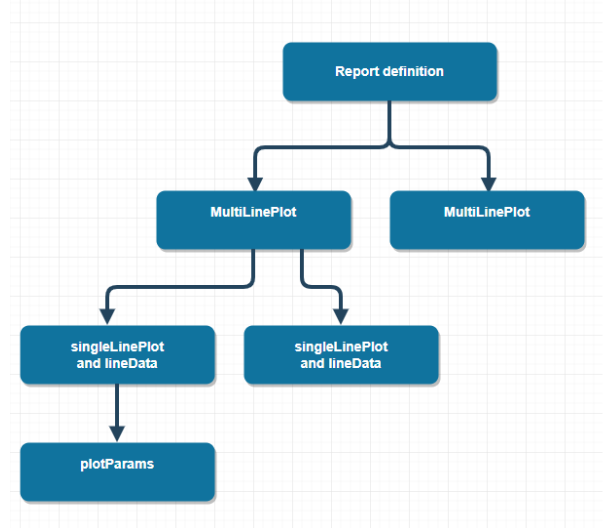
\includegraphics[scale=0.75]{pic/reportDefinitionStructure.png}
                    \caption{Struktura parametrů přicházejích z klientské části} \label{Obrázek č. 1}
                \end{figure}

    \subsection{API rozhraní}
        Zde je uveden seznam API rozhraní, které poskytuje potřebná data pro klientskou část aplikace. 
        \subsubsection*{SingleSeriesAveraged}
            Na základě těchto parametrů vrací časovou řadu a naní aplikovanou agregační funkci. Všechna fukncionalita je zajištěna servisním objektem SeriesService.
            \subsubsection*{Parametry akce}
                \begin{itemize}
                    \item DateTime From
                    \item DateTime To
                    \item TimeSpan Step
                    \item string SeriesName
                    \item int MeasurementPlaceNumberId
                \end{itemize}
                
        \subsubsection*{Export}
            Nejprve je vytvořena instance třídy MatplotLibCS s pomocí parametrů, kterými jsou cesty k souborům python.exe a matplotlib.py.
            Definice exportovaného dokumentu obsahujícího grafy je obsažena v parametru plotParams. Tento objekt je předám servisnímu objektu MatplotLibParamsMappingService, 
            který vytvoří validní strukturu parametrických objektů, které předá jako parametr instanci MatplotLibCS a zavolá metodu BuildFigure().
            \subsubsection*{Parametry akce}
                \begin{itemize}
                    \item MultilinePlotParams[] plotParams
                    \item string fileName 
                \end{itemize}

        \subsubsection*{SaveDashboardModel}
            Nástěnka složená z grafů je vytvořena na zákládě pole parametrických objektů MultilinePlotParams, které vznikají při přidávání grafů na nástěnku.
            Pokud si uživatel potřebuje aktuální nástěnku uložit, veškeré prametrické objekty se metodou post protokolu http odešlou na server, kde se serializují jako pole JSON
            a uloží do databáze do tabulky SavedDashboardModels.
            \subsubsection*{Parametry akce}
            \begin{itemize}
                \item MultilinePlotParams[] plotParams
                \item string name 
            \end{itemize}

        \subsubsection*{GetSavedDashboardModel}
            Podle parametru name vrátí uložený Dashboard model z tabulky SavedDashboardModels ve formátu JSON, 
            který si klientská aplikace deserializuje a podle nich vytvoří grafy v nástěnce.
            \subsubsection*{Parametry akce}
            \begin{itemize}
                \item string name 
            \end{itemize}

        \subsubsection{GetMessPlaces}
            Vrací seznam všech měřících míst. V aplikaci použito pro výběr měřícího místa. Tato akce nevyžaduje parametry.

        \subsubsection*{AllSeriesNames}
            Vrací seznam všech naměřených časových řad. V aplikaci použito pro výběr časové řady. Tato akce nevyžaduje parametry.

        \subsubsection*{GetSeriesUnit}
            V dtabázi v tabulce Units je ke každé časové řadě uložena jednotka v textovém formátu. 
            \subsubsection*{Parametry akce}
            \begin{itemize}
                \item string SeriesName
            \end{itemize}

    \section{Klientská část}
        Jedná se o javascriptovou aplikaci v technologii React ve spojení s MobX a Typescriptem.
        
        \subsection{Přístup k vývoji klientské aplikace}
            Objekty dělíme na vizuální komponenty a nevizuální objekty tzv. modely, 
            které slouží k obsluhám akcí uživatelského rozhraní a poskytování správných hodnot čtených visuálními komponentami.
            Díky MobX jsou hodnoty v komponentách vždy stejné jako v modelových třídách, 
            ze kterých komponenta příjmá proměnné pro prezentaci.
            Veškeré logické operace, volání api a výpočet hodnot by měl probíhat v modelových třídách. 
            Komponenty slouží pouze pro vizuální definici.

        \subsection{React Komponenty}
            Každá komponenta má object props definovatelného rozhraní, do kterého vstupují hodnoty z nadřazené komponenty, které se mají zobrazit.
            Dále každá komponenta musí implementovat metodu render(), kde je definováno jaká bude vizuální podoba komponenty.
            Každá komponenta může v metodě render() používat jiné komponenty, pokud jim předá správný objekt props.
            Na obrázku č. 5 vidíme kód jednoduché komponenty, která zobrazí předaný text.

        \subsection{MobX a modelové třídy}
            Modelové třídy vedle normálních atributů obsahují atributy s anotací @observable. 
            Hodnota těchto atributů bude vždy aktuální a stejná napříč celým stromem komponent, tam kde je čtena.
            Hlavním důvodem použití této technologie je její vliv na přívětivost aplikace a eliminace nevalidních stavů zobrazených hodnot.
            Dále je to hlavně uživatelská přívětivost a okamžitá odezva.
            Na obrázku č.6 vidíme kód jednoduchého použití MobX. Pokud hodnotu count změní jakákoliv komponenta volajíci akci increment, 
            změna se ihned projeví ve všech komponentách, které konkrétní model referencují.
        \subsection{Komunikace se serverem}
            Pro komnikaci se serverovým API jsem založil separátní třídu, ve které jsou všechny potřebné akce.
            Je zde použit balíček Fetch API \cite{29}, díky kterému lze snadno zkonstruovat libovolný požadavek na API.
            Na obrázku č. 7 vidíme zjištění jednotky veličiny podle názvu naměřené časové řady.
            \begin{figure}[h]
                \centering
                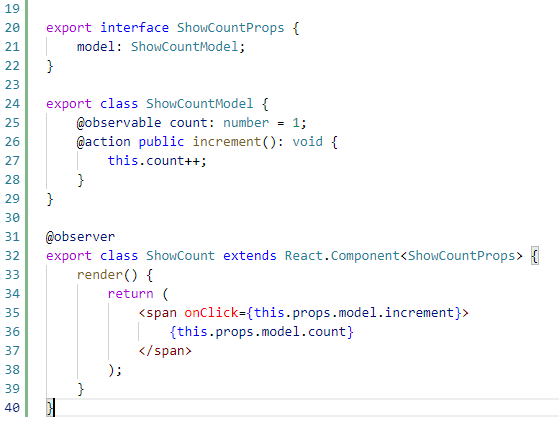
\includegraphics[scale=1]{pic/mobXexample.PNG}
                \caption{Příklad použití MobX} \label{Obrázek č. 6}
            \end{figure}

            \begin{figure}[h]
                \centering
                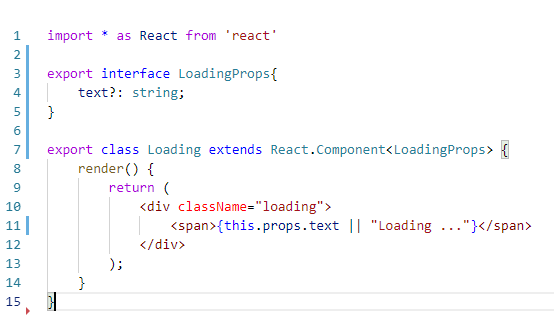
\includegraphics[scale=1]{pic/loadingComponentExample.PNG}
                \caption{Kód jednoduché komponenty v React} \label{Obrázek č. 5}
            \end{figure}
            \begin{figure}[h]
                \centering
                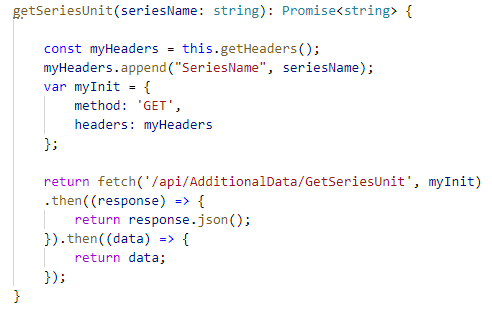
\includegraphics[scale=1]{pic/fetchexample.PNG}
                \caption{Příklad použití Fetch API} \label{Obrázek č. 7}
            \end{figure}

\chapter{Příklady analýz}
    \section{Porovnání činného a zdánlivého výkonu}
    Na obrázku č. 3.1 lze vidět porovnání průběhu zdánlivého a činného výkonu za jeden den.
    Vzhledem k fázovým posuvům mezi napětím a proudem v reálných obvodech střídavého proudu rozlišujeme tyto druhy výkonu:
        \subsection*{Zdánlivý výkon}
            Je dán součinem efektivních hodnot napětí a proudu. 
            Jedná se vlastně o celkový výkon obvodu. Značka S, jednotka VA (voltampér). 
        \subsection*{Jalový výkon}
            Jedná se o výkon ztrátový, tedy ten, který nevykonává žádnou práci. 
            Dochází u něj k výměně energie mezi elektrický polem obvodu a kondenzátoru nebo magnetickým polem cívky. 
            Ideální jalový výkon by se blížil k nule. Značka Q, jednotka (var).
        \subsection*{Činný výkon}
            Vyjadřuje efektivně využitou (spotřebovanou) el. energii, přeměněnou na jiný druh energie (mechanická, tepelná, a další). 
            Ideální činný výkon by se měl blížit k hodnotě zdánlivého výkonu. Značka P, jednotka W (watt). \cite{32}
        \begin{figure}[h]
            \centering
            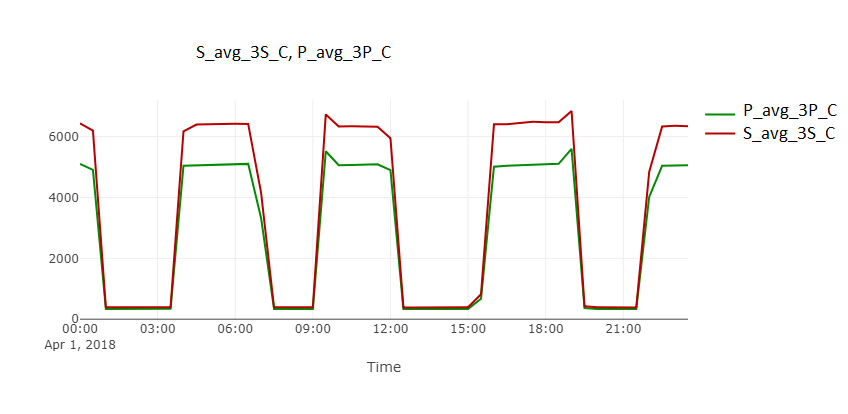
\includegraphics[scale=0.7]{pic/SP.png}
            \caption{Porovnání zdánlivého a činného výkonu za jeden den. Hodnoty jsou agregované po 30 minutách} \label{Obrázek č. 8}
        \end{figure}
        
    % \section{Porovnání poklesu napětí při sepnutí zátěže}
    %     Odchylka napětí rozvodů nízkého napětí s frekvencí 50 Hz je 230V. Měřené hodnoty se mohou lišit až o 10 \% od 
    %     jmenovité hodnoty. V praxi však tato jmenovitá hodnota napětí kolísá vlivem různých příčin. 
    %     Toto kolísání lze rozdělit na rychlé a pomalé změny napětí, které mohou být náhodné nebo pravidelné.
    %     Na obrázku č. 9 lze vidět jak pokleslo napětí při sepnutí zátěže.
    %     \begin{figure}[h]
    %         \centering
    %         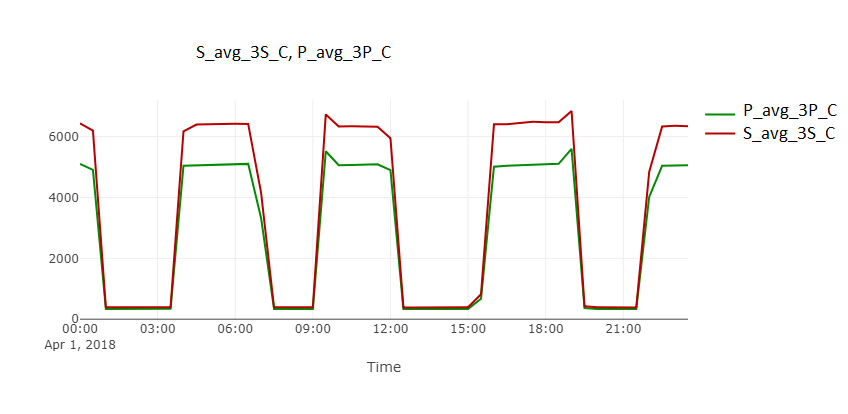
\includegraphics[scale=0.7]{pic/SP.png}
    %         \caption{Porovnání zdánlivého a činného výkonu za jeden den. Hodnoty jsou agregované po 30 minutách} \label{Obrázek č. 8}
    %     \end{figure}
    \section{Průměrování za daná období}
        Porovnání průběhů časové řady podle šířky intervalu pro použití agregační funkce průměrování. 
        Na obrázku č. 9 lze vidět průběh napětí průměrovaný po 1 hodině nahoře a po 10 minutách dole.
        \begin{figure}[h]
            \centering
            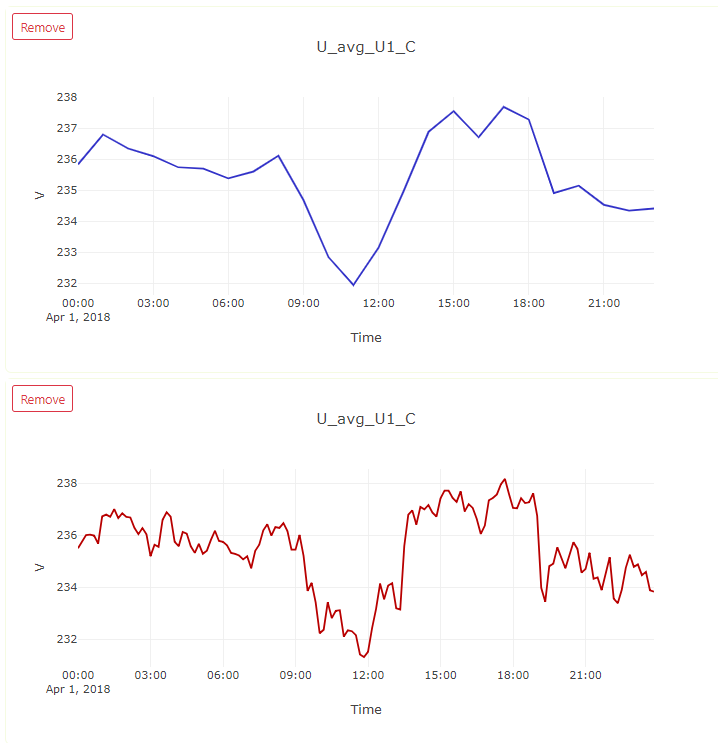
\includegraphics[scale=0.7]{pic/prumetovani.PNG}
            \caption{Porovnání agregační fuknce průměrování 1h a 10min.} \label{Obrázek č. 8}
        \end{figure}
    \section{Přehled spotřeby za dané období}
        Na obrázku č. 10 vidíme přehled průměrného zdánlivého výkonu za každý den v měsíci.
        \begin{figure}[h]
            \centering
            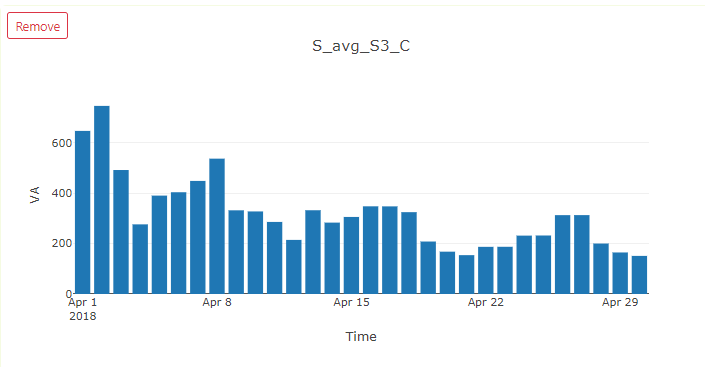
\includegraphics[scale=0.7]{pic/sko.PNG}
            \caption{Průměrný zdánlivý výkon pro každý den v měsíci} \label{Obrázek č. 8}
        \end{figure}

    % \section{Porovnání průběhu napětí s dlouhodbým průměrem}

\chapter{Pdf export}
    \section{Frontend export}
        Existují dva hlavní proudy javascriptových knihoven pro tvorbu pdf. 
        Prvním přístupem je tvorba pdf exportu toho co uživatel vidí v okně prohlížeče, či vybrané podčásti a jejich uložení jako obrázku do pdf, tzv. snapshot. 
        Sofistikovanější přístup nabízí například knihovny ReactPDF, PDFKit, či jsPDF, 
        které nabízí i možnost tvorby textového dokumentu s vloženými obrázky za pomoci vlastních subkomponent, například odstavec, stránka, citace, 
        které jsou nastavitelné pomocí kaskádových stylů, či parametrů konkrétních komponent.

        Zásadní nevýhodou exportovaného dokumentu a důvodem k nepoužití tohoto přístupu k ukládání reportů je nízká kvalita vložených grafů do exportovaného dokumentu, 
        rozmazanost, či jejich úplná absence. 
        Jelikož je graf v takovém dokumentu pouze bitmapový obrázek, nelze dokument kvalitně zvětšit, či přiblížit při prohlížení.

    \section{Backend export}
        Dokument je vytvářen na serveru za pomoci přijaté sady parametrů definujících výstupní objekt tak, 
        aby obsahoval grafy zobrazené na nástěnce v podobné fromě jako dokument pdf, který je vygenerován pomocí externí knihovny.

        Jednou z nevýhod použití tohoto přístupu je rozdílná vizuální podoba výstupu oproti frontend exportu, který funguje jako wysiwyg editor. 
        Formát a vzhled dokumentu lze definovat za pomoci omezené sady parametrů týkajících se převážně vzhledu grafů.

        Výhodou tohoto přístupu je možnost automatizovaného opakování tvorby dokumentů, které mohou být posílány automaticky klientům. 
        Grafy vytvořené knihovnami matplotlib, či gnuplot uložené do pdf jsou ve vektorové grafické podobě, tudíž je možno je libovolne zvětšit, či zmenšit.

\chapter{Návod ke spuštění aplikace}
    V přioženém CD ve složce SpecianBP nalezneme repozitář celého projektu. 
    Pro vývoj je možno projekt spustit pomocí vývojového prostředí Visual Studio 2017, kde stačí vybrat subprojekt WebUI a ten spustit. 
    Předpokladem spuštění aplikace je nainstalovaný .net framework core 2.2. 

    Před samotným spuštěním je nutné obnovit databázi z back-up souboru umístěného ve složce DBackup za pomoci Microsoft SQL Server Management Studio 2017.

    Po zkompilování se spustí serverová část aplikace, která po otevření ve webovém prohlížeči zobrazí klientskou část připravenou k použití. 
    Ta je již zkompilovaná a připravena k použití. Pro nahlédnutí do kódu klientské části aplikace lze použít libovlný textový editor.

    \section{Klientský dashboard}
        Po spuštění aplikace ve webovém prohlížeči vidí uživatel ovládací panel pro  přidávání grafů na nástěnku. 
        Přidávání grafů na nástěnku vytváří strukturu parametrických objektů ve formátu JSON, 
        která může být uložena pro budoucí zobrazení grafů bez nutnosti je znovu vytvářet a zároveň vidí výsledné grafy vytvořené z těchto parametrů.

        \begin{figure}[h]
            \centering
            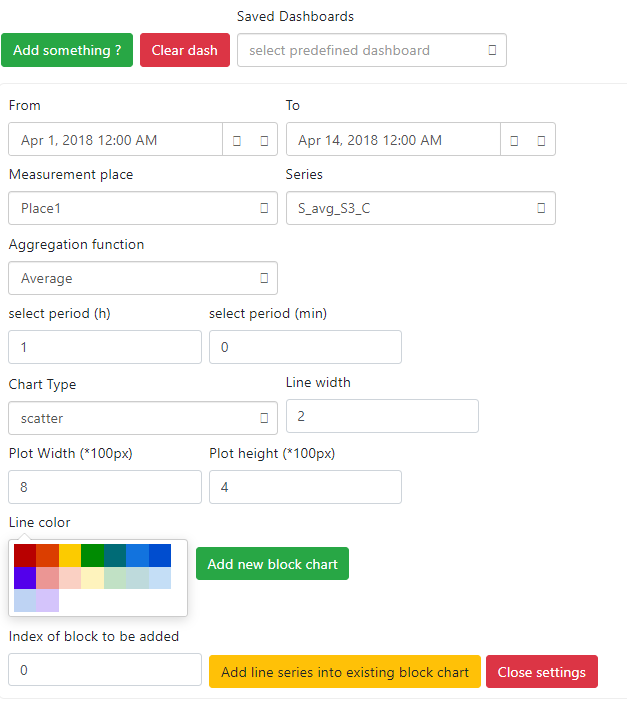
\includegraphics[scale=0.80]{pic/controlPanel.PNG}
            \caption{Ovládací panel pro přidávání grafů na nástěnku} \label{Obrázek č. 2}
        \end{figure}

        Uživatel může na nástěnku přidat libovolný počet komponent s grafem. 
        Každá grafová komponenta obsahuje průběh veličny ve zvoleném čase. 
        Lze vytvořit jeden graf s více průběhy pro porovnání.

        \subsection{Postup přidání grafu}
            Uživatel si vybere od kdy a do kdy a jakou časovou řadu podle názvu, dále měřící místo. Tyto vstupy jsou povinné.
            Agregační funkce může být libovolný časový interval v hodinách a minutách. Pokud je zvoleno nula hodin a nula minut, 
            agregační funkce se neaplikuje a serverová část vrátí časovou řadu ve všech naměřených hodnotách.

            Následně je možno vybrat typ grafu, barvu čáry, tloušťku čáry, pokud se jedná o spojnicový graf.
            Pak stačí graf přidat na nástěnku, či do již existujícího grafu.
        
            \begin{figure}[h]
                \centering
                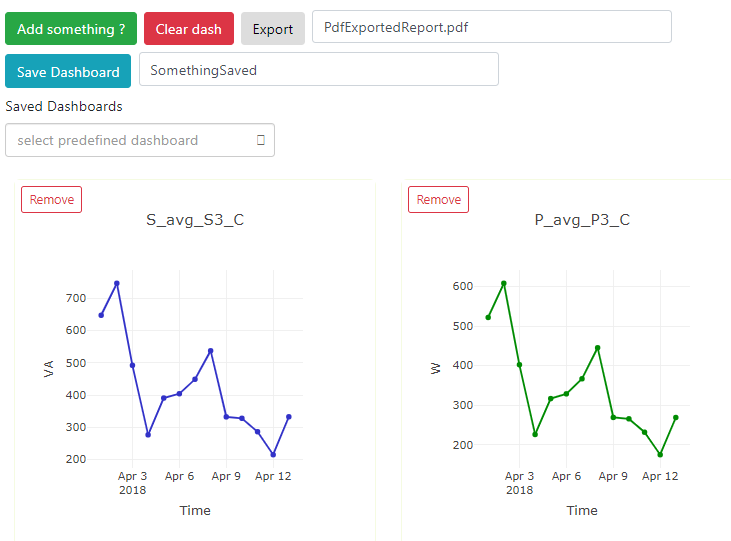
\includegraphics[scale=0.80]{pic/example1.PNG}
                \caption{Příklad nástěnky s dvěma grafy} \label{Obrázek č. 3}
            \end{figure}

        \subsection{Uložení nástěnky a export}
            Po vyplnění názvu exportovaného souboru lze exportovat grafy z nástěnky do pdf. 
            Stejně tak lze nástěnku uložit a po znovu supštění aplikace opět vyvolat.
            Takto uložená nástěnka je nástin definovatelného reportu, který kromě grafů obsahuje tabulky a text.
            
            \begin{figure}[h]
                \centering
                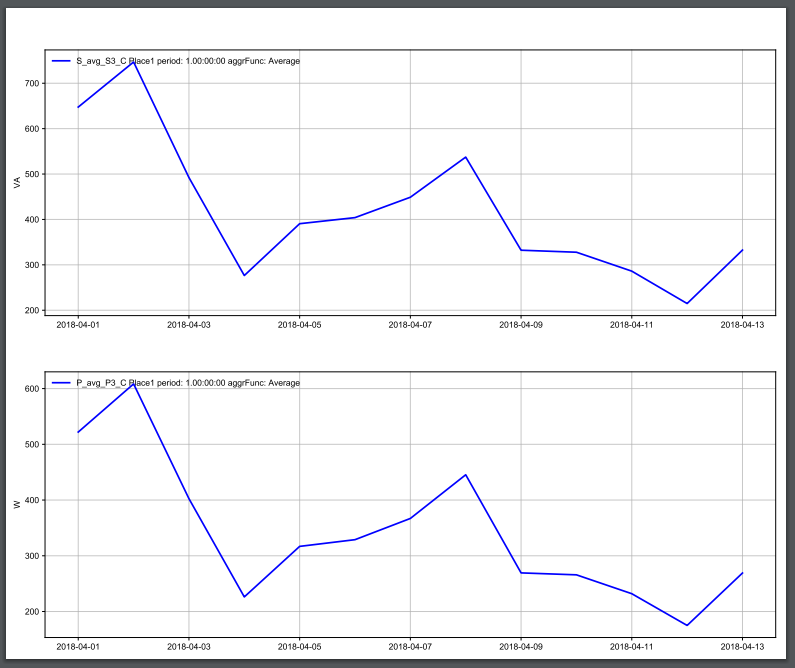
\includegraphics[scale=0.75]{pic/example1inPDF.PNG}
                \caption{Ukázka exportované nástěnky do pdf} \label{Obrázek č. 4}
            \end{figure}

\chapter{Závěr}
    \section{Dosažené výsledky}
        V rámci práce byly prozkoumány hodnoty uložené v archivech chytrého elektroměru, konkrétně v souborech ve formátu .CEA.
        Za pomoci knihoven KMB pro .NET Framework verze 4.5.2 byl přečten obsah archivů a převeden do relační databáze pro 
        snadný přístup k datům pomocí webové aplikace vyvíjené v .NET Core frameworku.

        Praktickým výsledkem mé práce je webová aplikace, která je schopná vizualizovat průběhy naměřených veličin v čase 
        pořízené chytrými elektroměry a tyto vizualizace zjednodušit pomocí agregačních funkcí při získávání časových řad z databáze.
        
        Zobrazení grafů probíhá podle předem definovatelných šablon v javascriptové grafové knihovně plotly.js.

        Serverová část poskytuje veřejné aplikační rozhraní pro libovolného klienta. Není zde nijak řešena autentifikace požadavků. 

        Vlastní migrace dat do relační databáze proběhla pouze pro demonstrační účely, 
        ale jinak není vhodná pro dlouhodobé ukládání měření stovek veličin periodicky. 
        Rychle roste její velikost
        Pro tuto bakalářskou práci byla poskytnuta data z chytrého elektroměru naměřena od 1.4.2018 do 1.9.2018. 
        Po migraci do relační databáze měl back-up soubor velikost 1.7GB. 
        Po přidání hodnot z více měřících míst stačí toto číslo vynásobit počtem měřících míst.
        Takto velký back-up soubor je velmi náročné obnovit v Microsoft SQL Management Studiu, jelikož to trvá velmi dlouho.
        V takto velké databázi pak dotazování se na časové řady pomocí sql se zpomaluje až na hranici smysluplné použitelnosti. 

        Díky CSS frameworku Bootstrap je vzhled aplikace responzivní a na první pohled přívětivý. 
        Při vložení velkého množství grafů na nástěnku webový prohlížeč nejevil známky zpomalení.
        Jelikož se při zavolání akce export odesílají pouze parametry nástěnky, jsou časové řady opět vybírány z databáze, 
        tudíž zde je nutné čekat v řádu jednotek sekund.

        Při vývoji aplikace jsem používal verzovací nástroj git, 
        který mi umožnil si v různých větvích držet různé funkční a nefunkční cesty vývoje 
        a spojovat do sebe různé věvte pro dosažení funkčního celku. \cite{27}
        Pro testování REST API jsem použil aplikaci PostMan. \cite{26}

    \section{Možnosti rozvoje tématu}
        \subsection*{Řízení uživatelů}
            V mé práci nebylo nijak řešeno řízení uživatelů, uživatelské profily, uživatelské role, autentifikace 
            a s tím spojená možnost každého uživatele vytvořit svou sadu definic pro reporty a být ve spojení se svými měřícimi přístroji.
            V současnosti probíhá ukládání definic (MultilinePlotParams objektů) a přístup ke všem datům pouze na globální úrovni.
            Řízení uživatelů považuji za další krok ve vývoji této aplikace nutný k jejímu dalšímu použití.
            
        \subsection*{Export report dokumentů}
            Definovatelný report by se měl skládat z tabulek, grafů a textu. 
            V aplikaci je to pouze sada grafů, které si uživatel definoval pomocí grafického uživatelského rozhraní.
            Bylo by vhodné nabídnout uživatelům i možnost exportu ve formátu csv.
        \subsection*{Automatický reporting}
            Nasazení a hlavní výhoda reportingu v praxi je automatická tvorba a odesílání například jako měsíční přehled, 
            notifikace k problému v síti, nebo na vyžádání za dané období.


\begin{thebibliography}{Mm99}
    \bibitem{1}
        ROTH, Daniel, Rick ANDERSON a Shaun LUTTIN, Introduction to ASP.NET Core [online]. Microsoft [cit. 2019-4-10]. Dostupné z: https://docs.microsoft.com/en-us/aspnet/core/?view=aspnetcore-2.2
    \bibitem{2}
        KURTZ, Jamie, 2013. ASP.NET MVC 4 and the Web API: building a REST service from start to finish. Berkeley, CA: Apress. Expert's voice in ASP.NET.
    \bibitem{3}
        Windows User Group [online]. Brno: dotNETcollege.cz, 2017 [cit. 2019-04-24]. Dostupné z: https://www.wug.cz/zaznamy/423-Programujeme-v-ASP-NET-Core-2-0
    \bibitem{4}
    https://docs.microsoft.com/cs-cz/ef/core/
    \bibitem{5}
    https://docs.microsoft.com/en-us/dotnet/csharp/programming-guide/concepts/linq/
    \bibitem{6}
    https://reactjs.org/ 
    \bibitem{7}
    http://jecas.cz/spa 
    \bibitem{8}
    https://mobx.js.org/getting-started.html
    \bibitem{9}
    https://www.npmjs.com/ 
    \bibitem{10}
    https://docs.npmjs.com/specifying-dependencies-and-devdependencies-in-a-package-json-file 
    \bibitem{11}
    https://www.typescriptlang.org/ 
    \bibitem{12}
    https://basarat.gitbooks.io/typescript/content/docs/why-typescript.html 
    \bibitem{13}
    https://plot.ly/javascript/react/ 
    \bibitem{14}
    https://medium.com/@alberto.park/a-simple-guide-how-to-select-a-chart-library-to-use-6f17878248f0
    \bibitem{15}
    https://medium.com/@ajmeyghani/javascript-bundlers-a-comparison-e63f01f2a364 
    \bibitem{16}
    https://webpack.js.org/guides/tree-shaking/ 
    \bibitem{17}
    https://parceljs.org/getting{\_}started.html 
    \bibitem{18}
    https://github.com/parcel-bundler/parcel 
    \bibitem{19}
    http://www.elektro.utb.cz/prednasky/prednaska7.pdf 
    \bibitem{20}
    http://elektrotechnika.chytrak.cz/files/dumy/10{\_}vykon{\_}AC.pdf 
    \bibitem{21}
    https://oenergetice.cz/elektrina/kvalita-elektricke-energie 
    \bibitem{22}
    http://www.odbornecasopisy.cz/elektro/casopis/tema/jak-rychle-nalezt-zdroj-ruseni-poklesu-a-vypadku-napeti-na-vedeni--14330 
    \bibitem{23}
    https://docs.microsoft.com/cs-cz/ef/core/managing-schemas/migrations/
    \bibitem{24}
    https://babeljs.io/docs/en/learn/
    \bibitem{25}
    https://docs.microsoft.com/cs-cz/aspnet/core/fundamentals/dependency-injection?view=aspnetcore-2.2
    \bibitem{26}
    https://www.getpostman.com/collection
    \bibitem{27}
    https://gitforwindows.org/
    \bibitem{28}
    https://github.com/ITGlobal/MatplotlibCS
    \bibitem{29}
    https://developer.mozilla.org/en-US/docs/Web/API/Fetch{\_}API/Using{\_}Fetch
    \bibitem{30}
    https://dspace.cvut.cz/handle/10467/74218
    \bibitem{31}
    https://dspace.cvut.cz/bitstream/handle/10467/76218/F3-BP-2018-Cabrova-Lucia-Zavedeni%20systemu%20energetickeho%20managementu.pdf?sequence=-1&isAllowed=y
    \bibitem{32}
    http://www.elektro.utb.cz/prednasky/prednaska7.pdf 
\end{thebibliography}

\end{document}
